\chapter{Theoretical and Architectural Basis}

This chapter establishes the theoretical foundations necessary for the
development of the proposed solution. It begins by contextualizing Software
Architecture within dynamic and agile environments, identifying the friction
between rapid delivery and architectural integrity. Subsequently, it delineates
the central problem motivating this work: the dissonance between distributed
team structures and centralized decision-making methods. To address this gap,
the chapter introduces the concept of Internal Developer Portals (IDPs) as
essential infrastructure for team autonomy. Finally, it details the principles
of Hypothesis Engineering and the ArchHypo framework, justifying the necessity
for specific tooling to operationalize these practices.

\section{The Role of Software Architecture in Agile and High-Flow Environments}

Software Architecture (SA) is a fundamental concept in software development,
forming the structural foundation of systems and ensuring their long-term
sustainability. While early definitions characterized SA as a composition of
elements, form, and rationale, modern definitions have evolved to incorporate
deeper insights into the dynamics of system evolution. Contemporary definitions
characterize SA as a high-level system structure encompassing essential
characteristics, design principles, and the decisions to guide system
adaptability and maintainability.

This expanded perspective highlights that SA is not merely a static blueprint
but a dynamic framework that guides decisions throughout the system life cycle
and aligns technical and business needs. However, the practical application of
architectural design is fraught with complexity, particularly regarding the
timing and certainty of decisions.

\subsection{The Challenge of Architecture in Agile Contexts}

Agile methodologies have successfully introduced practices like Test-Driven
Development (TDD) and refactoring, yet they often lack well-recognized and
agreed-upon approaches for architectural design. In many agile contexts, the
most recognized approach is to simply let the architecture emerge and refine it
over the life of the project. While this approach aims to reduce upfront
design, it often leads to a lack of established practice, meaning architectural
changes remain challenging within agile contexts, often necessitating
significant upfront design that contradicts core agile principles.

In rapidly evolving business environments, such as software startups, new
requirements continually reshape architectural demands. In these dynamic
scenarios, architecture anti-patterns—such as the "Big Ball of Mud"—may emerge,
posing risks to effective architectural evolution and resulting in systems that
struggle to maintain proper modularity and scalability.

This anti-pattern often emerges when immediate demands and incremental fixes
override deliberate architectural planning. Consequently, engineering teams
must balance speed with quality to ensure sustainable, adaptable architectures
that meet evolving business demands.

\subsection{Trends in Evolutionary Architecture}

To address the friction between agility and structure, concepts such as
\textit{Agile Architecture} and \textit{Continuous Architecture} have emerged.
These frameworks emphasize principles such as delaying design decisions and
architecting for change. The core philosophy is that decisions can be postponed
until they are absolutely necessary, ensuring that architectures are based on
facts rather than guesses.

However, determining which decisions to delay or where flexibility is
beneficial incurs significant challenges. Time emerges as a critical dimension
in architectural design, with iterative planning being essential, particularly
for solutions undergoing continuous evolution.

\subsection{The Necessity of Fast Flow}

Recent industry trends emphasize the concept of fast flow, which refers to an
organization's ability to continuously and rapidly deliver software changes
that align with evolving business needs while preserving the system health and
architectural integrity. Achieving fast flow relies on autonomous, empowered
teams supported by self-service platforms that minimize operational blockers.

This concept is intrinsically linked to the adoption of socio-technical
architecture, which reflects the growing realization that architectural
decisions should not be confined to a select few architects but distributed
across development teams. The socio-technical approach promotes team autonomy
and empowerment, advocating for decision-making processes that include all team
members, regardless of their experience levels.

\section{The Dissonance in Architectural Decision-Making}

Despite the industry's aspiration for decentralized, autonomous teams capable
of maintaining a fast flow of requirements, a significant theoretical and
practical barrier exists. We identify this barrier as the operational gap
between intent and method.

\subsection{The Conflict: Autonomy vs. Tacit Knowledge}

A fundamental conflict exists between industry reports advocating for
decentralized, team-driven architectural decisions and academic research
indicating that existing methods for deriving SA still heavily depend on the
tacit knowledge of experienced practitioners.

While the industry moves toward distributed architectural ownership, the
current methods and frameworks continue to reinforce centralized
decision-making. This creates a self-reinforcing cycle: while organizations may
aim for a decentralized approach to support a fast flow of requirements, they
remain dependent on expert-driven methods that, by design, limit the
involvement of less experienced team members.

\subsection{Reliance on Tacit Knowledge}

A systematic mapping study by \cite{SysMap} examined methods and practices for
deriving architectural models from requirements specifications. A key finding
was that existing methods strongly relied on experienced practitioners' tacit
knowledge to derive the architectural definitions for a software system. This
reliance on the intuition and expertise of architects makes it difficult for
teams without such expertise to adopt these methods effectively.

This dependency creates bottlenecks that limit an effective decentralization of
decision-making. As a result, the shift towards a more distributed
decision-making model is obstructed by frameworks that inherently require
centralization, blocking the practical adoption of a socio-technical
architecture approach.

\subsection{Deficiencies in Existing Methods}

Beyond the reliance on tacit knowledge, the systematic mapping study
highlighted several other gaps in existing architectural derivation methods:

\begin{itemize}
	\item \textbf{Lack of Tool Support:} About a third of analyzed architectural derivation approaches lack tool support. The study noted that only 30.7\% of methods provided decision-making support.
	\item \textbf{Inadequate Support for Non-Functional Requirements (NFRs):} Although NFRs such as performance, scalability, and security are essential, many approaches focus primarily on functional requirements, neglecting NFRs in architectural decision-making processes.
	\item \textbf{Limited Empirical Validation:} Many methods have not been sufficiently validated in real-world, dynamic environments. Over half lack explicit evaluation methods.
\end{itemize}

This points to a clear need for tools to aid architects, suggesting patterns
and supporting decision-making to reduce dependency on seasoned experts.

\section{Internal Developer Portals and Backstage}

To bridge the gap between autonomous teams and the complex ecosystem of modern
software development, the industry has turned toward \textit{Platform
	Engineering} and the implementation of Internal Developer Portals (IDPs).

\subsection{The Role of Developer Portals}

An Internal Developer Portal (IDP) serves as the primary interface between
developers and the underlying platform infrastructure. Unlike a simple wiki or
a project management tool, an IDP is an operational hub that aggregates tools,
services, documentation, and data into a unified "pane of glass."

The primary goal of an IDP is to reduce cognitive load. By abstracting the
complexity of infrastructure and standardizing workflows, IDPs enable "Golden
Paths"—recommended, supported, and automated paths for building and deploying
software. This aligns directly with the goal of decentralized architecture:
providing teams with the autonomy to build and own their services while
ensuring governance and best practices are baked into the tooling.

\subsection{Backstage: The Open Platform for Building Developer Portals}

Backstage is an open-source framework for building Internal Developer Portals
(IDPs), originally developed by Spotify and now hosted by the Cloud Native
Computing Foundation (CNCF). Due to its extensibility and "catalog-first"
philosophy, it has emerged as the de facto standard for developer portals.

\subsubsection{Architecture and Core Components}

As illustrated in Figure~\ref{fig:backstage}, Backstage is not a rigid
application but rather a modular ecosystem driven by configuration. The
architecture is divided into several key interaction layers:

\begin{itemize}
	\item \textbf{The Core Framework:} The central hub of the application which manages essential utilities such as the \textit{Plugin Loader}, \textit{Router}, \textit{Auth Service}, and \textit{Error Handling}. It acts as the bridge between the configuration and the varied plugins.
	\item \textbf{Plugin Ecosystem:} Backstage relies heavily on a split-plugin architecture:
	      \begin{itemize}
		      \item \textbf{Frontend Plugins:} Handle Views, UI Components, and API Clients to present data to the user.
		      \item \textbf{Backend Plugins:} Manage API Services, Data Processing, and Storage, communicating directly with the core framework.
	      \end{itemize}
	\item \textbf{External Integrations:} The Backend Plugins serve as the gateway to \textit{External Systems \& APIs}, allowing the portal to aggregate data from cloud providers, CI/CD tools, and other infrastructure.
\end{itemize}

\begin{figure}
	\centering
	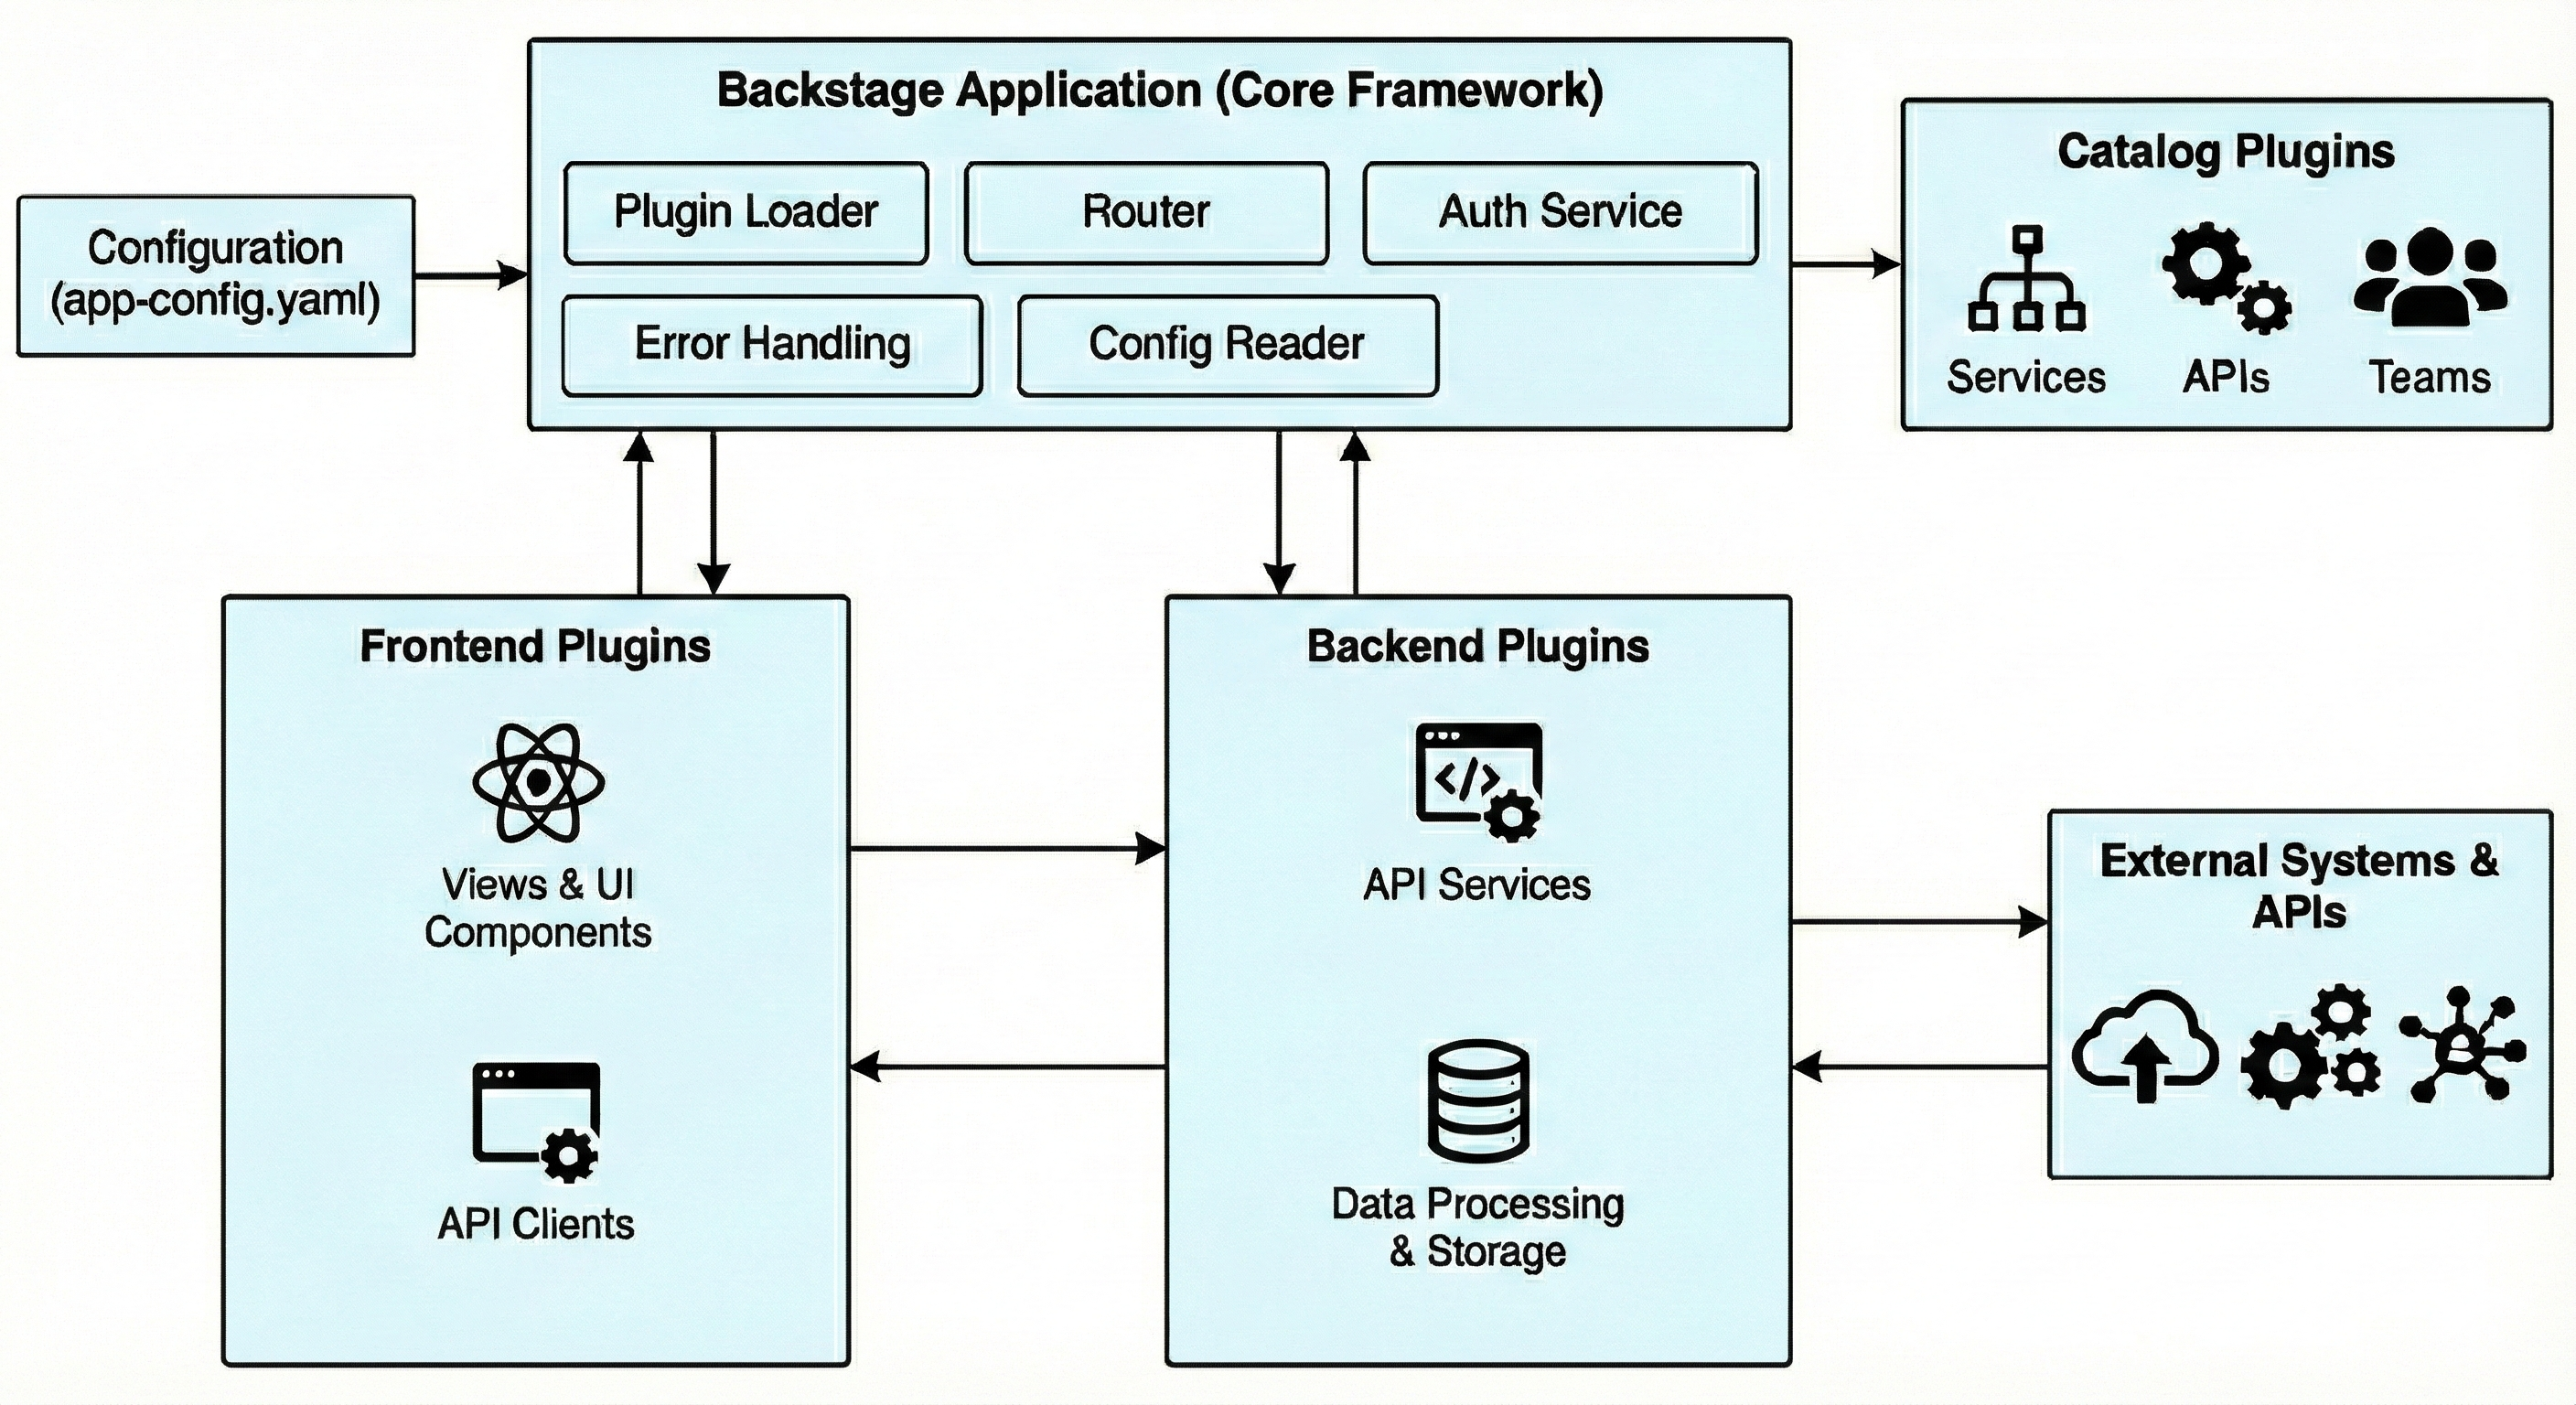
\includegraphics[width=0.9\textwidth]{contents/images/backstage}
	\caption{The Backstage organization and platform structure}
	\label{fig:backstage}
\end{figure}

Crucially, Backstage is built on a plugin architecture. This allows
organizations to extend the portal's functionality by integrating custom tools
directly into the developer's daily workflow without forcing developers to
switch contexts.

\section{Hypothesis Engineering and Uncertainty Management}

To resolve the decision-making gap and enable decentralized architecture, it is
necessary to move away from reliance on tacit intuition toward a more explicit
management of the unknowns. This is achieved through \textbf{Hypothesis
	Engineering}.

\subsection{The Concept of Hypothesis Engineering}

Hypothesis Engineering offers a philosophical approach to managing uncertainty
by treating assumptions as testable hypotheses. It is defined as a process of
continuously validating product assumptions, transforming them into hypotheses,
prioritizing and testing them following the scientific method to support or
refute them.

In this context, the word "hypothesis" focuses on business assumptions that
should be evaluated before start-ups develop their business models. However,
this concept is extended here to manage the uncertainty of architectural
decisions.

\subsection{Distinguishing Uncertainty from Risk}

A critical theoretical distinction must be made between \textbf{risk} and
\textbf{uncertainty}. Risk involves evaluating the probability and impact of
specific events; it represents the likelihood of an event occurring and its
potential consequences.

In contrast, \textbf{uncertainty} refers to the lack of information necessary
for architectural decisions. Uncertainty represents the lack of information to
make a decision; in cases where partial information is available, the
uncertainty is related to what is still unknown. ArchHypo is based on the
premise that uncertainties related to the software architecture are natural in
all stages of a software project and that, instead of resisting them, a better
approach would be to embrace and manage them.

\subsection{Characteristics of an Architectural Hypothesis}

An architectural hypothesis represents any uncertain statement relevant to the
software architecture design. Its primary characteristic is that it must be
\textbf{falsifiable}—that is, the possibility of proving it false exists.

Unlike a requirement statement, which is usually assumed as true when written,
using the word hypothesis makes it clear to the whole team that it represents
uncertainty. Hypotheses must be shared with the development team so that
everyone is aware of the uncertainties that can affect architectural decisions.
This explicit documentation allows the team to systematically test and validate
assumptions, gather data, and adjust their approach as needed.

\section{The ArchHypo Framework}

ArchHypo is a technique that uses hypothesis engineering to manage
uncertainties related to software architecture and enhance decision-making
processes. It provides a structured framework for software architects and
developers, enabling them to make uncertainties explicit and manageable.

\begin{figure}
	\centering
	\includegraphics[width=0.9\textwidth]{contents/images/archhypo-lifecycle-crop}
	\caption{The ArchHypo decision management lifecycle}
	\label{fig:archhypo-lifecycle}
\end{figure}

\subsection{Sources of Uncertainty}

When applying ArchHypo, a team focuses specifically on hypotheses that can
affect the software architecture. The most common sources of uncertainty are in
the \textbf{requirements} and the \textbf{solutions}.

\begin{itemize}
	\item \textbf{Requirements Uncertainty:} This occurs when a requirement is based on limited evidence or lacks important details. For instance, uncertainty regarding the number of simultaneous requests a system must handle.
	\item \textbf{Solution Uncertainty:} This relates to the unknown consequences of current architecture components or candidate solutions. For example, uncertainty regarding whether a specific library is compatible with a required protocol.
\end{itemize}

\subsection{Assessment: Uncertainty Level and Impact Level}

Once a hypothesis is identified, it is assessed based on two independent
dimensions:

\begin{itemize}
	\item \textbf{Uncertainty Level:} This reflects how far the team is from proving that a hypothesis is true or false. The uncertainty would be high if there is a lack of information to estimate probability or when alternatives have a similar chance to happen.
	\item \textbf{Impact Level:} This measures the effort required to transition to a different alternative. It represents the consequences and costs that the uncertainty can cause.
\end{itemize}

This assessment is typically performed qualitatively by the team, using a scale
(e.g., a five-point Likert scale: Very Low to Very High). These assessments aim
to provoke reflection about the hypotheses, allowing a qualitative comparison
among them and helping in choosing techniques for handling the respective
uncertainty.

\subsection{The Technical Plan}

The core operational mechanism of ArchHypo is the formulation of a
\textbf{Technical Plan} based on each hypothesis' assessment. This plan is
derived from the pattern \textit{Plan for Responsible Moments}.

The plan can include actions aiming to:

\begin{itemize}
	\item Definitely accept or refute the hypothesis.
	\item \textbf{Reduce the uncertainty:} Giving the team more confidence to move forward with a decision.
	\item \textbf{Reduce the impact:} Allowing the team to stay longer with the uncertainty by isolating the affected areas or increasing flexibility.
	\item Define criteria (triggers) to postpone handling the hypothesis until a specific
	      condition is met.
\end{itemize}

\subsection{Supporting Practices and Patterns}

The technical plan utilizes a specific pattern language to address
uncertainties. Key patterns include:

\begin{itemize}
	\item \textbf{Architectural Spike:} Small technical experiments in which working software is created to prove or disprove the feasibility of a specific hypothesis.
	\item \textbf{Tracer Bullet:} An architecturally significant functionality that helps to exercise and demonstrate an end-to-end path inside the architecture, aiming to evaluate how new technologies could be integrated. This pattern provides a concrete way to design the basic application architecture.
	\item \textbf{Software Analytics:} Identifying relevant metrics to collect and analyze to assess and monitor a given quality attribute of the system.
	\item \textbf{Architectural Trigger:} Defines conditions that trigger architectural investigations which may lead to adding tasks to the backlog. For example, having a given number of simultaneous accesses might fire a trigger related to scalability.
	\item \textbf{Development Guidelines:} Small adjustments in the development process to deal with recurrent uncertainties.
	\item \textbf{Protective Guideline:} Defining programming practices to be followed or avoided to not limit options for an architectural decision being postponed.
	\item \textbf{Bring the Specialist:} Involving individuals with the right skills or knowledge in activities where this expertise can reduce the uncertainty.
	\item \textbf{Plan for Preparation:} Introducing steps to obtain information before activities that recurrently have an associated uncertainty.
	\item \textbf{Quality Checkpoint:} Introducing a verification activity after the development of an artifact to verify if the desired quality is present.
\end{itemize}

\section{The Practical Gap and the Need for Tooling}

While the theoretical framework of ArchHypo is robust, empirical evidence
suggests that its manual application presents significant challenges that
hinder widespread adoption.

\subsection{Adoption Barriers}

The empirical study in \cite{ArchHypo} found that, although the technique
offered a structured approach to dividing architectural work, the team
identified significant challenges in its adoption due to the learning curve and
required process adjustments. In particular, participants reported difficulty
in learning the method, especially with respect to mapping risks, specifying
hypotheses, and defining action plans.

Team members mentioned difficulty in mapping the scenarios with risk to the
hypothesis and definition of the actions to handle the hypothesis. One
participant explicitly noted that "train[ing] the team a little more on how to
find, map risk scenarios, and define the necessary actions... would make the
team less dependent on the team of architects".

\subsection{The Integration Necessity}

The identified difficulties highlight a strong need for better guidance and,
crucially, \textbf{tool support to manage hypotheses and execute action plans}.
However, standalone tools often suffer from low adoption because they require
developers to leave their primary workflow.

This justifies the decision to integrate ArchHypo into an IDP like Backstage.
By embedding hypothesis management into the same platform where developers
already manage services, documentation, and deployments, we can reduce the
cognitive load of adoption. This integration—operationalized in the proposed
\textbf{HypoStage} plugin—aims to bridge the gap between theoretical agility
and the practical reality of fast-paced development.
